% title section ================================================================
\begin{center}
    \large
    \textbf{Thesis Proposal: Using a Modified Point Net to \\ Generate 3D Bounding Box Proposals with Stereo Disparity Maps}\\
    \noindent \textbf{April-August 2019}\\
    \normalsize 
\end{center}

\begin{tabular}{ll}
    Student: & Kristian Gonzalez \\
    & Ravensburg-Weingarten University of Applied Sciences\\
    Supervisor: & Prof. Dr. Wolfgang Ertel \\
    & Ravensburg-Weingarten University of Applied Sciences\\
    Co-supervisor: & Prof. Dr. Stefan Elser\\
    & Ravensburg-Weingarten University of Applied Sciences\\
\end{tabular}

% body section =================================================================

% intro ========================================================================
\section{Introduction} 
%delme: things to talk about:
%	a little about computer vision
%	what are typical issues in field
%	what is main problem?
%	small sample of solution (to be intro'd later) \\
%% %%%%%%%%%%%%%%%%%%%%%%%%%%%%%%%%%%%%%%
Computer vision is a field that has grown explosively in the last few years, very much in thanks to the utilization of convolutional neural networks, or CNN's, to accurately identify different kinds of information from raw image data. This capability has led to many different sub-fields of research, including 3D localization of objects using a variety of sensor setups. In having a branching set of possible sensor setups, a few questions naturally arise: how many sensors are needed to accurately locate objects, and how competitive are systems that do not directly take distance measurements to localize objects? 

In the field of autonomous driving, a ``typical" sensor system may include any combination of the following: forward facing camera, a complimentary second camera for stereo image generation, an IMU (inertial measurement unit), a lidar sensor (either a single sensor on the top or one at the front \& back of the vehicle), a forward-facing radar, and possibly other cameras facing various directions. The KITTI dataset \cite{geiger_are_2012} features one lidar sensor with multiple cameras; the Oxford RobotCar \cite{maddern_1_2017}, which focuses on driving through a similar area multiple times, especially contains two lidar sensors (front and rear); finally, some datasets such as Apolloscape \cite{huang_apolloscape_2018} or Berkeley Deep Drive \cite{yu_bdd100k:_2018} obtain large amounts of RGB data, with less of a focus on lidar or stereo imaging. 

Because of this sensor complexity, this paper proposes to seek out a more streamlined approach by primarily utilizing stereo vision to create 3D bounding box proposals and estimates. The current norm in the field leans heavily towards using lidar-based networks (typically nets that use some combination of camera and lidar information), while this paper instead asks: can stereo disparity maps provide a competitive alternative by using methods adapted from lidar networks? It must be acknowledged at the start of this proposal that lidar sensors do typically provide more accurate distance measurements by virtue of directly measuring the environment, but not without downsides. Lidar technology is typically expensive (although this price is decreasing), and has difficulty with reflective surfaces. Therefore, the aim of this paper is not to obtain better 3D object detection than lidar, but to demonstrate stereo vision's competitiveness. 

To that end, this paper proposes a novel method of using stereo disparity maps to localize objects. A modified stereo depth estimation network, Pyramid Stereo Matching Network (PSMnet), will be used to generate a stereo image, which will then be projected to 3D point space and fed into a well-known point network, Frustum Point Net (FPnet).


% related work =================================================================
\section{Related Work}

\subsection{Convolutional Networks Using Point Clouds}
A variety of networks exist that estimate 3-dimensional bounding boxes, including Frustum Pointnet, which is to be modified in this paper. FPnet takes a three step approach, which includes: ``traditional" 2D object detection, 3D segmentation, and amodal estimation. This is demonstrated below in Figure \ref{FpGenSteps}, reproduced from the original paper.
\begin{figure}[ht] % h = "approx here", {h,t,b}
    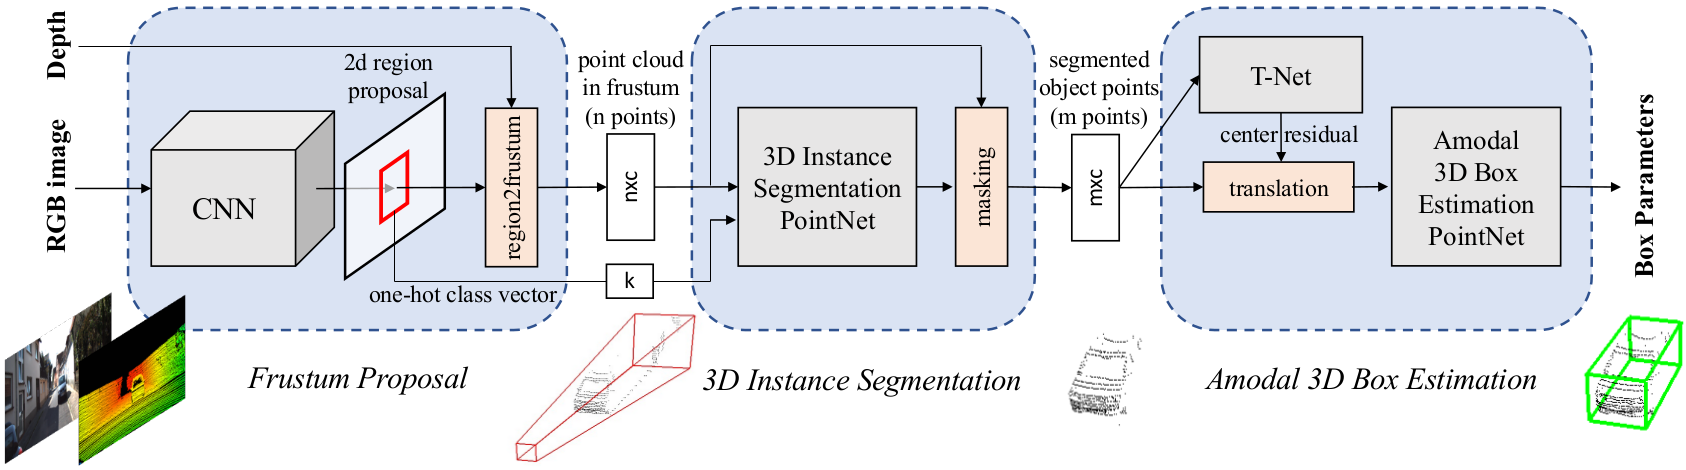
\includegraphics[width=1\textwidth]{m/fpnet_steps.png}
    \label{FpGenSteps}
    \caption{Reproduced image of general FPnet steps. First, 2D object detection locates an image and creates a ``frustum" (or cone) of the valid lidar point cloud. Next, this reduced set of points segmented in the 3D space, by removing the fore- and background points. Finally, an estimate of the remaining points is made about the object's size and orientation to generate a bounding box.}
% \label{figure-parking}
\end{figure}


The first point net to successfully implement this approach was the aptly-named ``Pointnet" \cite{qi2017pointnet}, which focused on working with point cloud data in its native format, rather than transform the data to 3D voxel grids or views. This approach provides some clear advantages over networks like Voxnet \cite{maturana2015voxnet}, which relies on creating a three-dimensional occupancy grid requiring a reference frame and given resolution. Though creating volumetric or 3D CNN's created an initial approach, they are limited by data sparsity and computation cost. By contrast, the original Pointnet and subsequent FPnet are designed to work with a point cloud's inherent properties, paraphrased from \cite{qi2017pointnet}: 
\begin{itemize} \itemsep=-0.5em
    \item Unordered: point clouds are essentially an unordered set of vectors containing \textit{x,y,z} coordinates, among other information.
    \item Point interaction: because the points come from euclidean space, neighboring points form a meaningful group, so any network must be able to represent the ``local structures" of a subset of points.
    \item Invariance under transformation: some simple transformations, such as rotation, translation, or scaling, do not change the inherent category the object belongs to, such as a car or plane.
\end{itemize}

Using multiple views is another approach taken to tackle point cloud data. In practice, multi-view CNN's project 3D point clouds onto 2D planes, then apply 2D CNN's for classification. However, this rapidly increases in complexity when extending the usage to understanding or shape completion. 

\subsection{Using CNN's to Generate Stereo Disparity Maps}
Creating a disparity map by use of two cameras, or stereo matching,has its roots in finding a matching pixel between two cameras to understand its distance away from the cameras by use of epipolar geometry. Typically, an image similar to Figure \ref{stereo_intro} (reproduced from Hamzah and Ibrahim \cite{hamzah_literature_2016}) below is used to illustrate this. 

\begin{figure}[ht] % h = "approx here", {h,t,b}
    \centering
    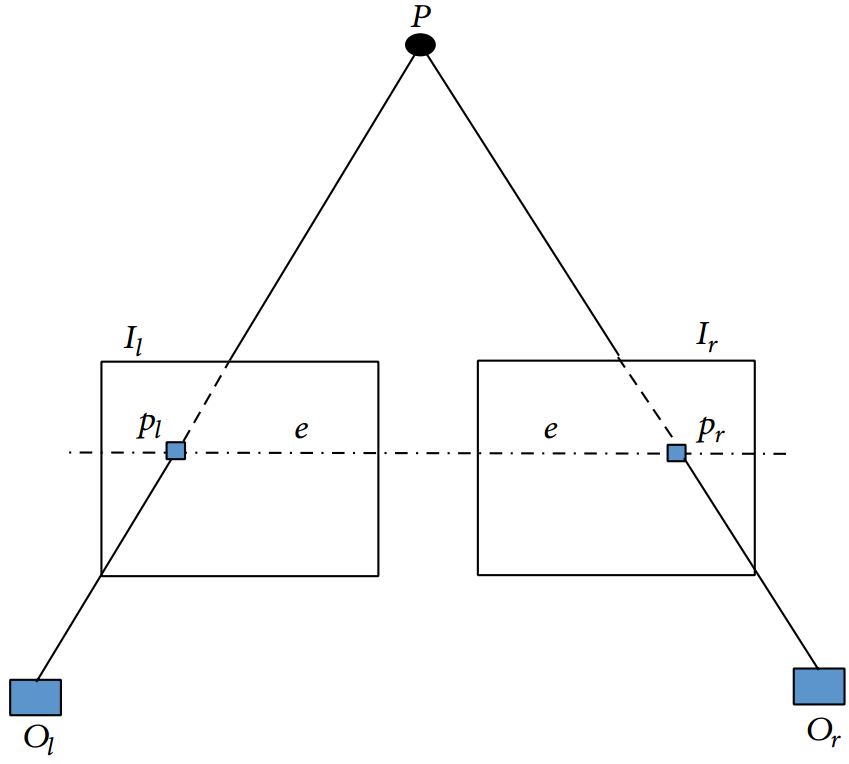
\includegraphics[width=0.35\textwidth]{m/stereo_parallax.png}
    \label{stereo_intro}
    \caption{Using trigonometry, a target at point P can be located on two image planes at their local points and estimated at a certain distance from the sensors.}
    % \label{figure-parking}
\end{figure}

Ibraim and Hamzah \cite{hamzah_literature_2016} present a comprehensive but not exhaustive survey on existing algorithms, several of which used only a CPU for their calculations. However, as also stated, the ``number of calculations required increases with an increasing number of pixels", making the matching problem computationally complex. Of course, any discussion of stereo correspondence algorithms warrants mention of the four classical steps of stereo matching, per \cite{scharstein2002taxonomy}: matching cost computation, aggregation, optimization, and refinement.

To know the state of the art of stereo disparity map creation, one may look at various benchmarks that use a single, common dataset to compare multiple networks and algorithms. The well-known Middlebury \cite{scharstein2014high,middlebury_leaderboard} dataset is a common benchmark, as well as the KITTI \cite{geiger_are_2012,kitti_stereo_board} 2015 Stereo benchmark. Additionally, there are even some aggregate lists, including the 2018 Robust Vision Challenge \cite{rvc_leaderboard} leaderboard. Looking at the aggregated Robust Vision Challenge leaderboard, last updated in December 2018, two top-performing networks are iResNet, holding 1st place, as well as PSMnet (Pyramid Stereo Matching network), in 4th place. What also makes these two stereo networks special is that both have publicly available repositories. Furthermore, PSMnet, or Pyramid Stereo-Matching Network, has simpler and fewer dependencies than iResNet. Lastly, PSMnet is (as of this writing) in the top 10 of the current KITTI 2015 stereo vision challenge leaderboard. 

PSMnet itself is comprised of two main modules, as stated by the authors: spatial pyramid pooling and a 3D CNN. The overall architecture, reproduced from the original paper, is shown below in Figure \ref{PsmGenSteps}. 

\begin{figure}[ht] % h = "approx here", {h,t,b}
    \centering
    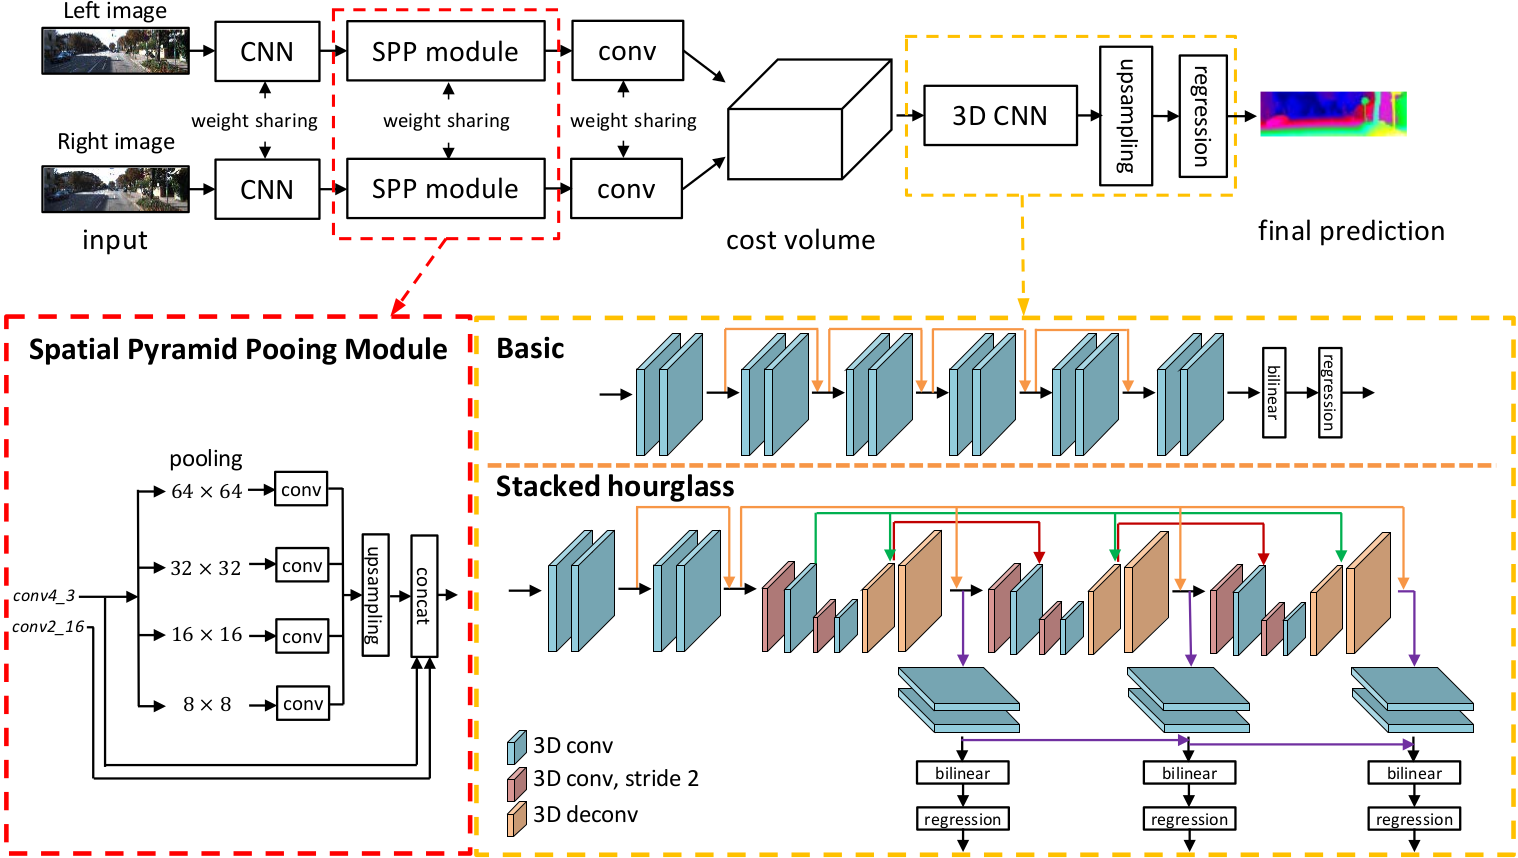
\includegraphics[width=1\textwidth]{m/psmnet_steps.png}
    \label{PsmGenSteps}
    \caption{Reproduced from original paper \cite{chang_pyramid_2018}. Two main components, spatial pyramid pooling (harvests features) and a 3D CNN (regularizes cost volume / performs disparity regression) form the basis of the network.}
    % \label{figure-parking}
\end{figure}

An interesting note on the spatial pyramid pooling module is how it addresses fixed-size constraint in CNN's. At various dimensional sizes, feature maps are generated and flattened, which are then fed into a fully connected classification layer. Finally, these features are compressed via adaptive average pooling, then upsampled back to the original feature map size, leaving a multi-level feature map for consumption of the 3D CNN.

\subsection{Using Stereo Disparity Maps and CNN's for 3D Object Detection}
%kjgnote: need some examples of networks that have been developed for stereo-based 3D localizations should check a few sources, including: 
%* kitti dataset
%* oxford robotcar
%* cityscapes
%* what other benchmarks are there?
%
%from kitti benchmark:
%* Stereo R-CNN

%1. read stereo rcnn 
%2. make a list of s-rcnn's related works, investigate those
%3. look at fpnet and check for stereo nets
%4. look at a non-kitti benchmark (cityscapes)


There is a relatively small body of literature on stereo-based 3D object detection. As of the time of this writing, Li et al. \cite{li2019stereo} created the only stereo-based network on the 3D KITTI Vision Benchmark, Stereo R-CNN. This network is inspired by Faster R-CNN and also features weight sharing and a region proposal network. What sets this network apart is how it predicts object keypoints, which are then used in 3D box estimation. Each image stream has a stereo RPN (region proposal network with shared weights, which is then processed with an ROI Align operation; each ROI pair is then used to generate the relevant keypoints via ``photometric alignment", or more specifically the left region of interest is warped to reduce the photometric error, leading to find the ``best center depth".

Chen and Kundu \cite{DBLP:journals/corr/ChenKZMFU16} make a primary assumption that all relevant classes are on the ground plane, and ``only depth information (no appearance)" is used in the 3D object proposal generation process. Additionally, each object proposal is taken from a set of templates, learned in the training data to represent the typical size of each class, requiring some a priori information.

% proposal =====================================================================
\section{Proposed Solution}
%delme: things to talk about: 
%	what is your general approach
%	how is each part to be prepared
%	how will results be verified?
%	what are your expected risks?
%	what is expected timeline of project \\
%% %%%%%%%%%%%%%%%%%%%%%%%%%%%%%%%%%%%%%%

Given the current state of 3D localization using stereo vision, as well the opportunity it presents, this paper proposes to investigate taking a new approach on 3D localization using stereo data. The key idea is to use inspiration from Frustum Pointnet, taking a point cloud and working with that data in 3D space rather than 2D space, and extend this to stereo data. Using an appropriate transform, disparity data that is projected onto the 2D image plane can be moved to 3D space, and treated as a point cloud. With this pseudo-point cloud, generated from a best-in-class stereo algorithm such as Pyramid Stereo Matching, Frustum Pointnet will be trained and evaluated on its performance with this new data input. 
Naturally, there are several moving components in this idea, and each must be addressed: 
\begin{itemize}\itemsep=-0.5em
    \item Obtaining stereo disparity maps from PSMnet
    \item Transforming between lidar data and stereo data
    \item Feeding this data into FPnet
    \item Evaluating performance on 3D bounding boxes
    \item Overall Project Timeline
\end{itemize}

\subsection{Obtaining stereo disparity maps}
In order to obtain stereo disparity maps, Pyramid Stereo Matching has been selected to output this data. The networks is easily one of the best in its class, and has openly available code. In fact, this network has already been downloaded, configured, and modularized as of the time of this writing. This means that the important first step of obtaining stereo images from the dataset has been completed. Additionally, this means that the network has been simplified down to a simple object that can be called: the loaded model is given a stereo image pair and returns an estimated disparity map. The model was trained following the instructions by the original authors: first it was trained from scratch on Freiburg SceneFlow data for 10 epochs, then finetuned on KITTI 2015 stereo data for 300 epochs. This has thus produced a ready-to-use solution for stereo imaging using the KITTI dataset. 

\subsection{Transforming between Lidar Data and Stereo Data}
The task of transforming stereo data into a point cloud (and perhaps the reverse as well) is also underway, and already has some initial results. There are some important steps required to transform a stereo image into something that can imitate a point cloud, but a side-by-side comparison of two similar images may provide some insight. There are technically two datasets being demonstrated below from KITTI benchmark, the stereo 2015 dataset and the 3D object detection dataset. As seen below in Figure \ref{stereo_comparison}, there are some visual correlations between a transformed image (c) and the stereo ground truth (d).


\begin{figure}[ht]
    \centering  
    \subfigure[LHS image, Object detection dataset]{
        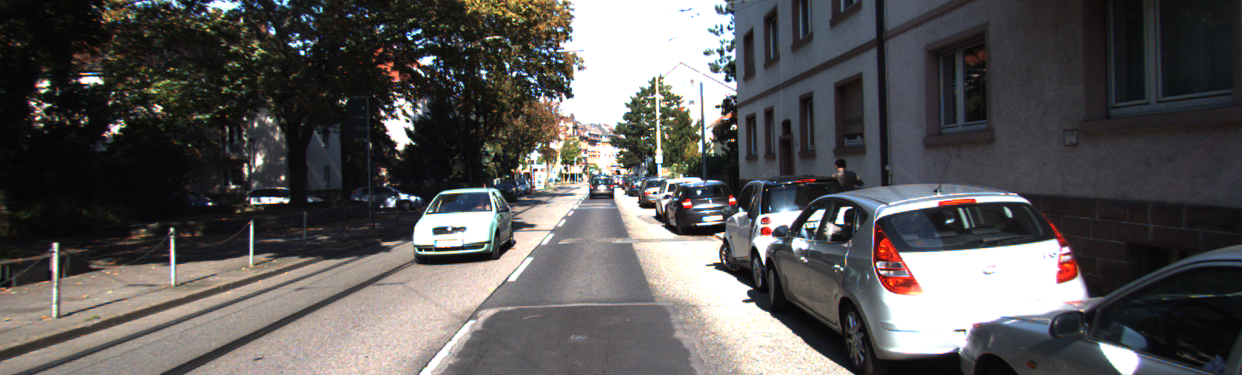
\includegraphics[width=0.45\linewidth]{m/000286_lhs_objdet.png}}
    \subfigure[LHS image, Stereo dataset]{
        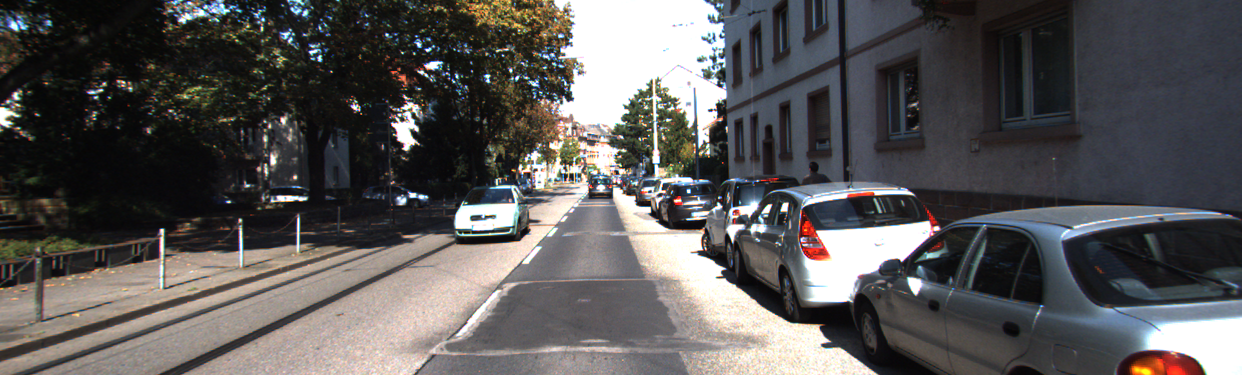
\includegraphics[width=0.45\linewidth]{m/000132_10_lhs_stereo.png}}
    \subfigure[Projected Lidar, Object Detection]{
        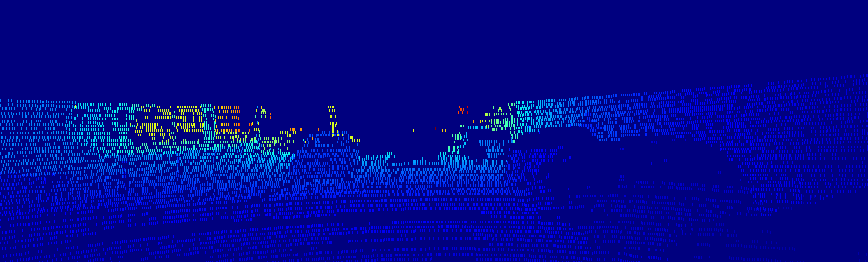
\includegraphics[width=0.45\linewidth]{m/000286_disp_gen.png}}
    \subfigure[Disparity Ground Truth, Stereo]{
        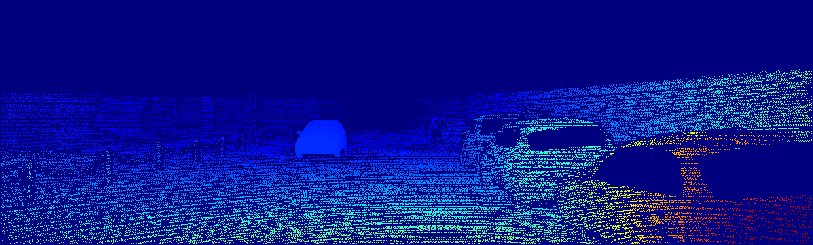
\includegraphics[width=0.45\linewidth]{m/000132_10_disp_gt.png}}
    \label{stereo_comparison}
    \caption{Side-by-side comparison of similar images from different datasets and their respective depth images. Sub-figure (c) was created by taking the record's lidar scan and projecting the points onto the image plane. By contrast, Sub-figure (d) is the stereo dataset record's ground truth image, and seems to have higher values for points that are closer. }
\end{figure}

This aspect of the project, while important, is expected to take some time to develop a suitable transformation function, but should feature simpler mathematics by comparison. The main task is not to identically match each pixel that lidar and stereo data share, but rather to reduce error as much as possible so that the difference between stereo and lidar performance is not due to the conversion between one format to the other.

\subsection{Feeding Data into FPnet}
In order to modify the data going into Frustum Pointnet, there must be some understanding of how to interact with the original data. This step may take some iteration, but is expected to be understood within the first half of the thesis. The original author's repository for FPnet uses Tensorflow, different than the PyTorch implementation of Stereo Pyramid Matching. This means that there will generally be some slowdown when converting from one format to another, but there is no back-propagation that will be performed from one network to the other. The primary idea here is that FPnet will receive either a stereo disparity map or a pseudo-point cloud that comes from a previously trained, fully functioning stereo generation network. Thus, FPnet will take the data as-is, and learn to estimate distance from these values.

\subsection{Evaluating Performance on 3D Bounding Boxes}
In order to properly evaluate the detections of the network's 3D bounding boxes, the well known methods of evaluating 2D bounding boxes must be adapted. This has already been investigated and implemented by David Stutz and Bo Li \cite{kitti_3d_board}. Thus, this method will be followed to evaluate and compare performance of the network. If other, more accurate methods become available in the course of the project, they will be used instead.

\subsection{Project Timeline}
In order to meet all requirements while also satisfying educational program requirements, a proposed timeline is provided below. Notable dates here include the official start of the thesis, the final date of the thesis, including presentation and document turn-in.

% kjgnote: "makebox" used in order to make an oversized-but-still-centered figure
\begin{figure}[h] % ahh, h = "approx here", t = "top of page", b = "bottom of pg"
    \makebox[\textwidth][c]{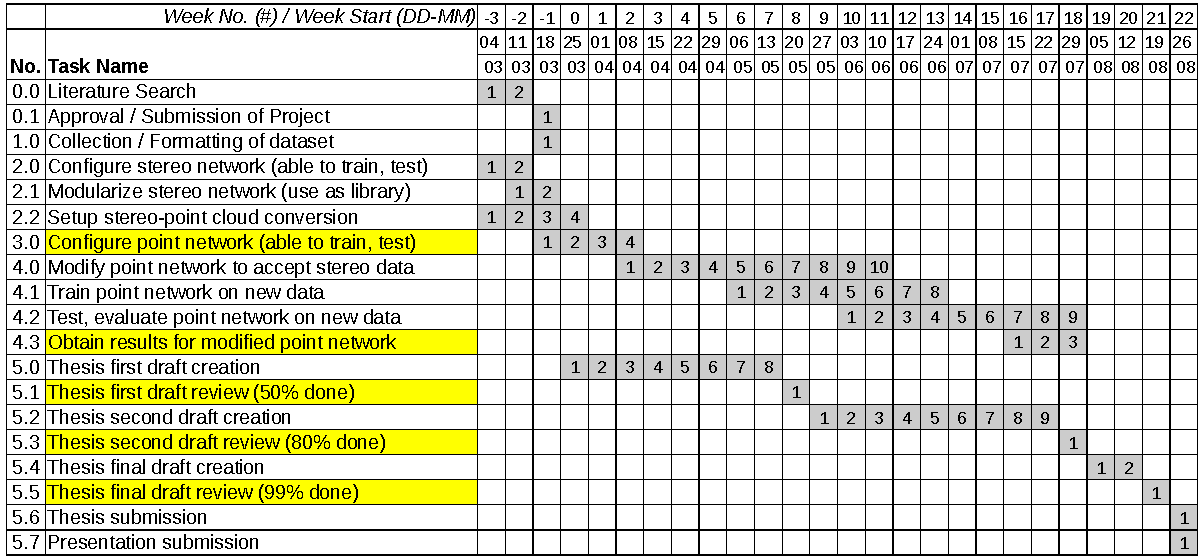
\includegraphics[scale=.85]{m/proposed_timeline.pdf}}
    \caption{Proposed schedule of paper. Highlighted tasks are critical milestones. Numbers inside of gray cells indicate the number of weeks each individual task lasts.}
% \label{figure-parking}
\end{figure}

\newpage

% eof
